\begin{frame}[fragile]{Textbooks using Julia}
    
\pause

\begin{columns}

  \begin{column}{0.30\textwidth}
    \centering
    \begin{tikzpicture}
        \node[draw=white, line width=1pt, inner sep=0pt] {
            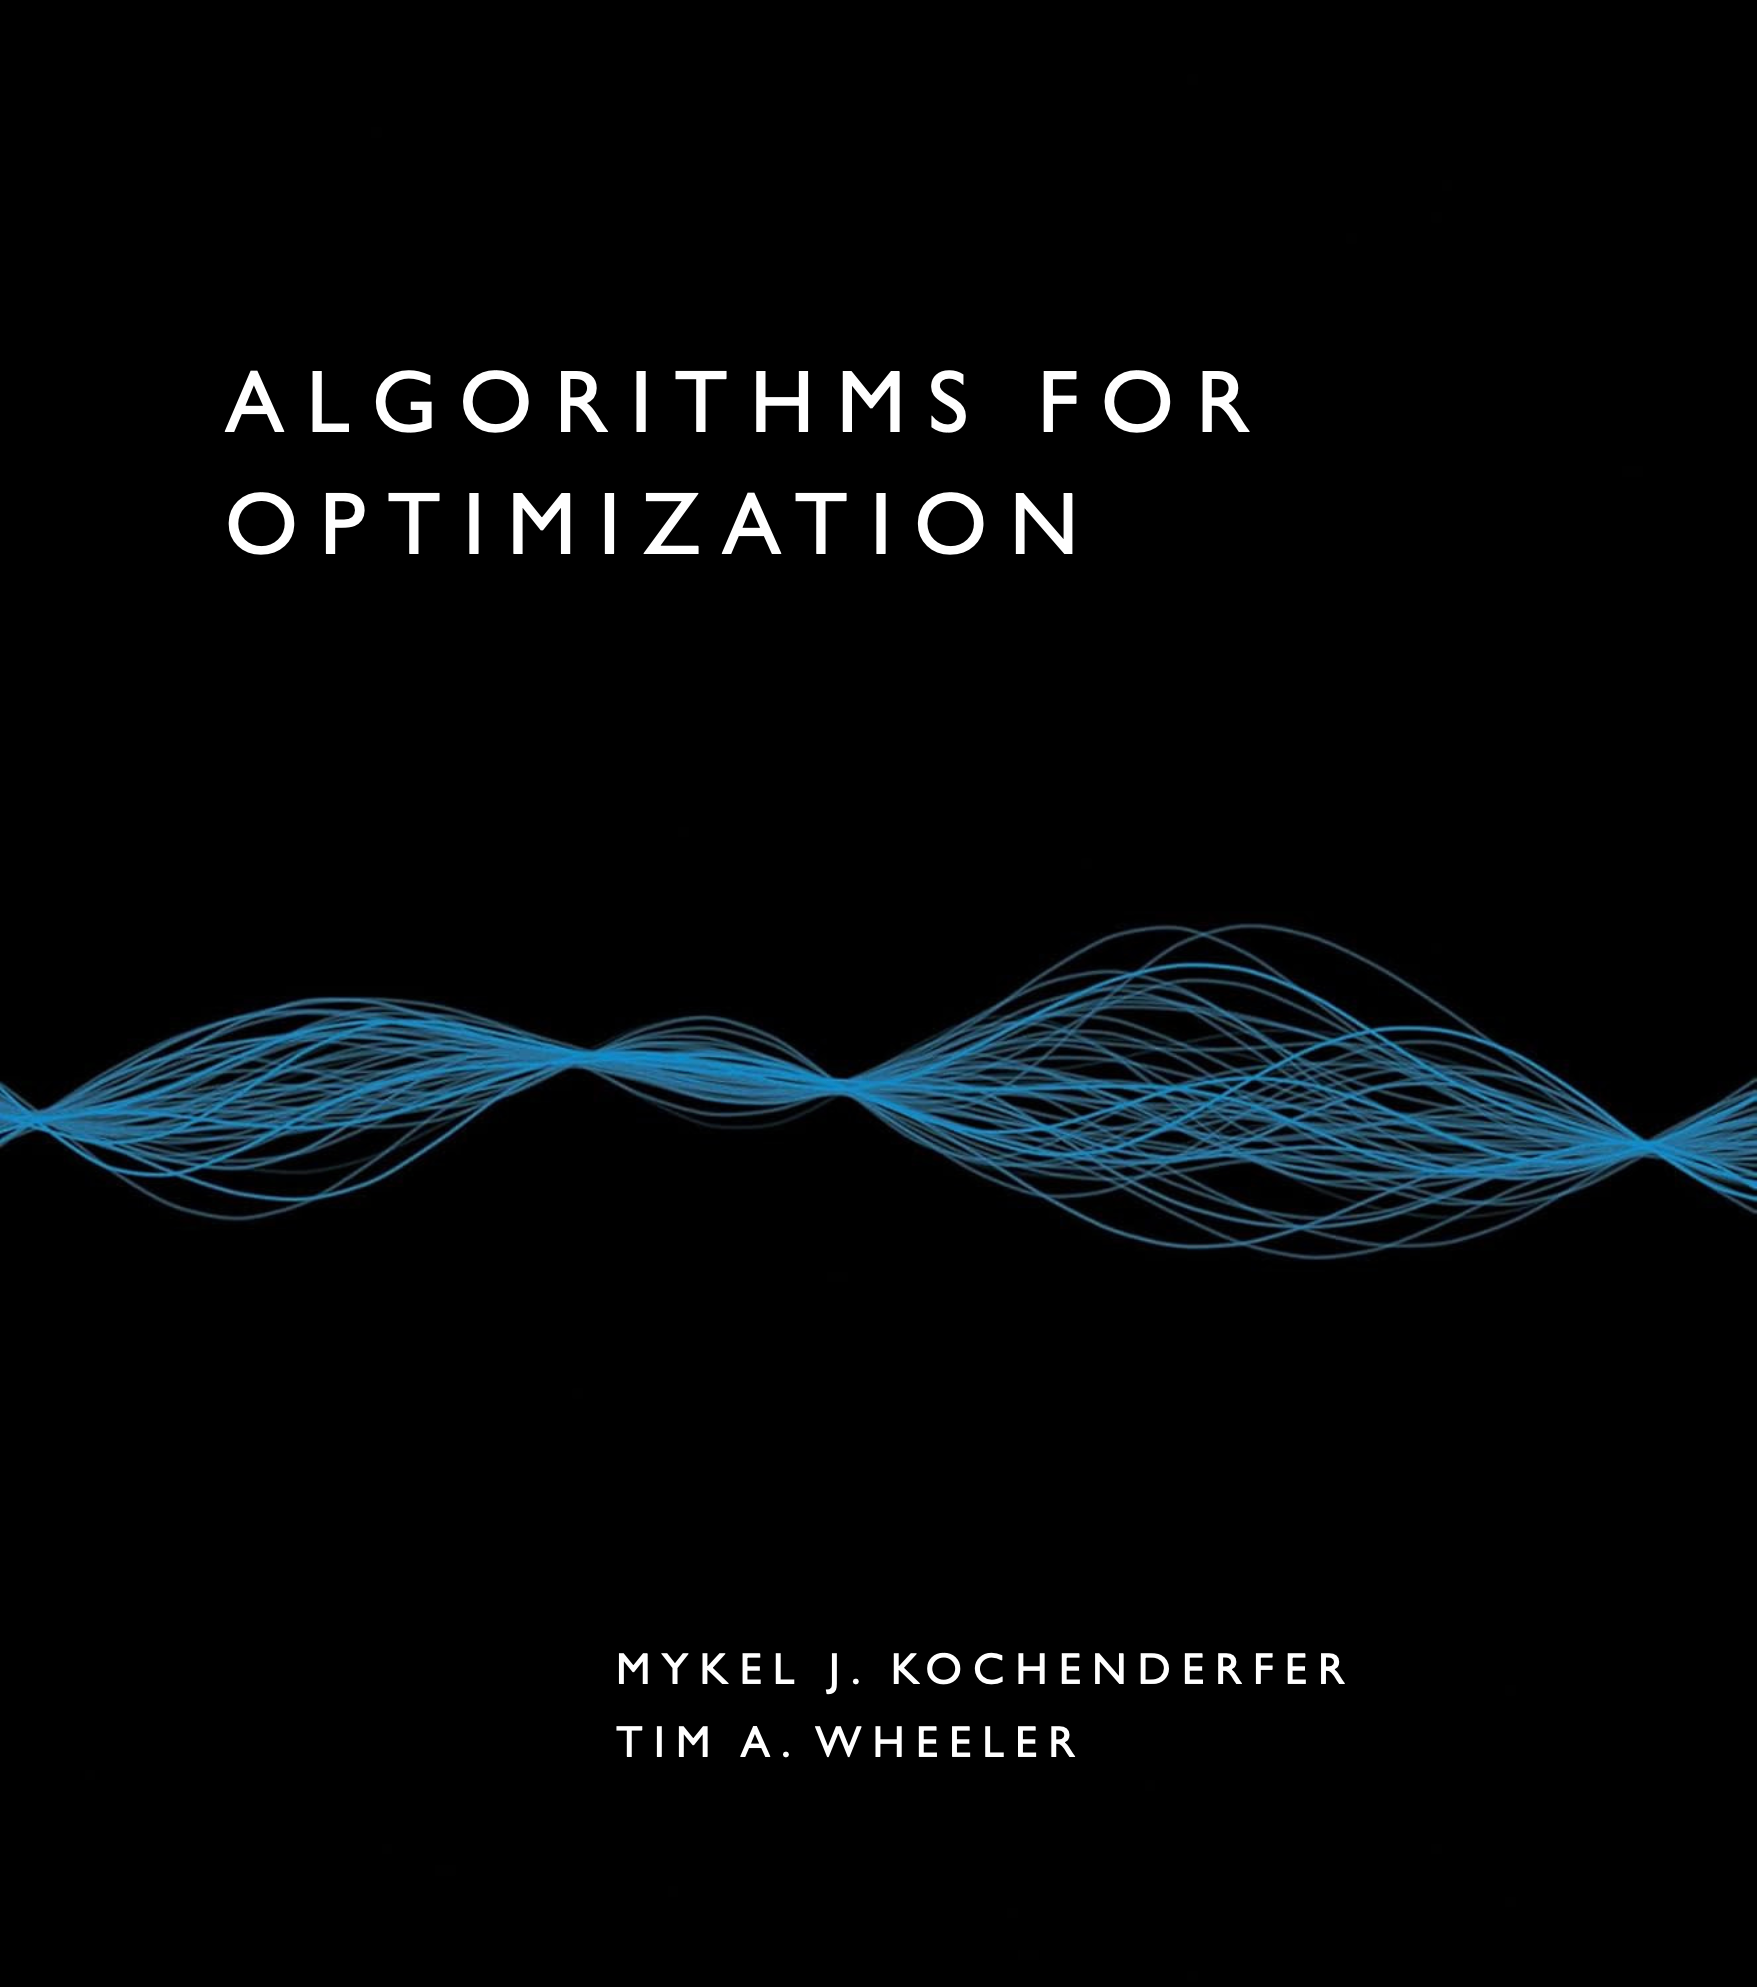
\includegraphics[width=\linewidth]{media/algforopt.png}
        };
    \end{tikzpicture}
    
    \captionof*{figure}{\shortstack{\footnotesize Algorithms for Optimization\\\textcolor{gray}{\scriptsize MIT Press, 2019}}}
  \end{column}

  \pause

  \begin{column}{0.30\textwidth}
    \centering
    \begin{tikzpicture}
        \node[draw=white, line width=1pt, inner sep=0pt] {
            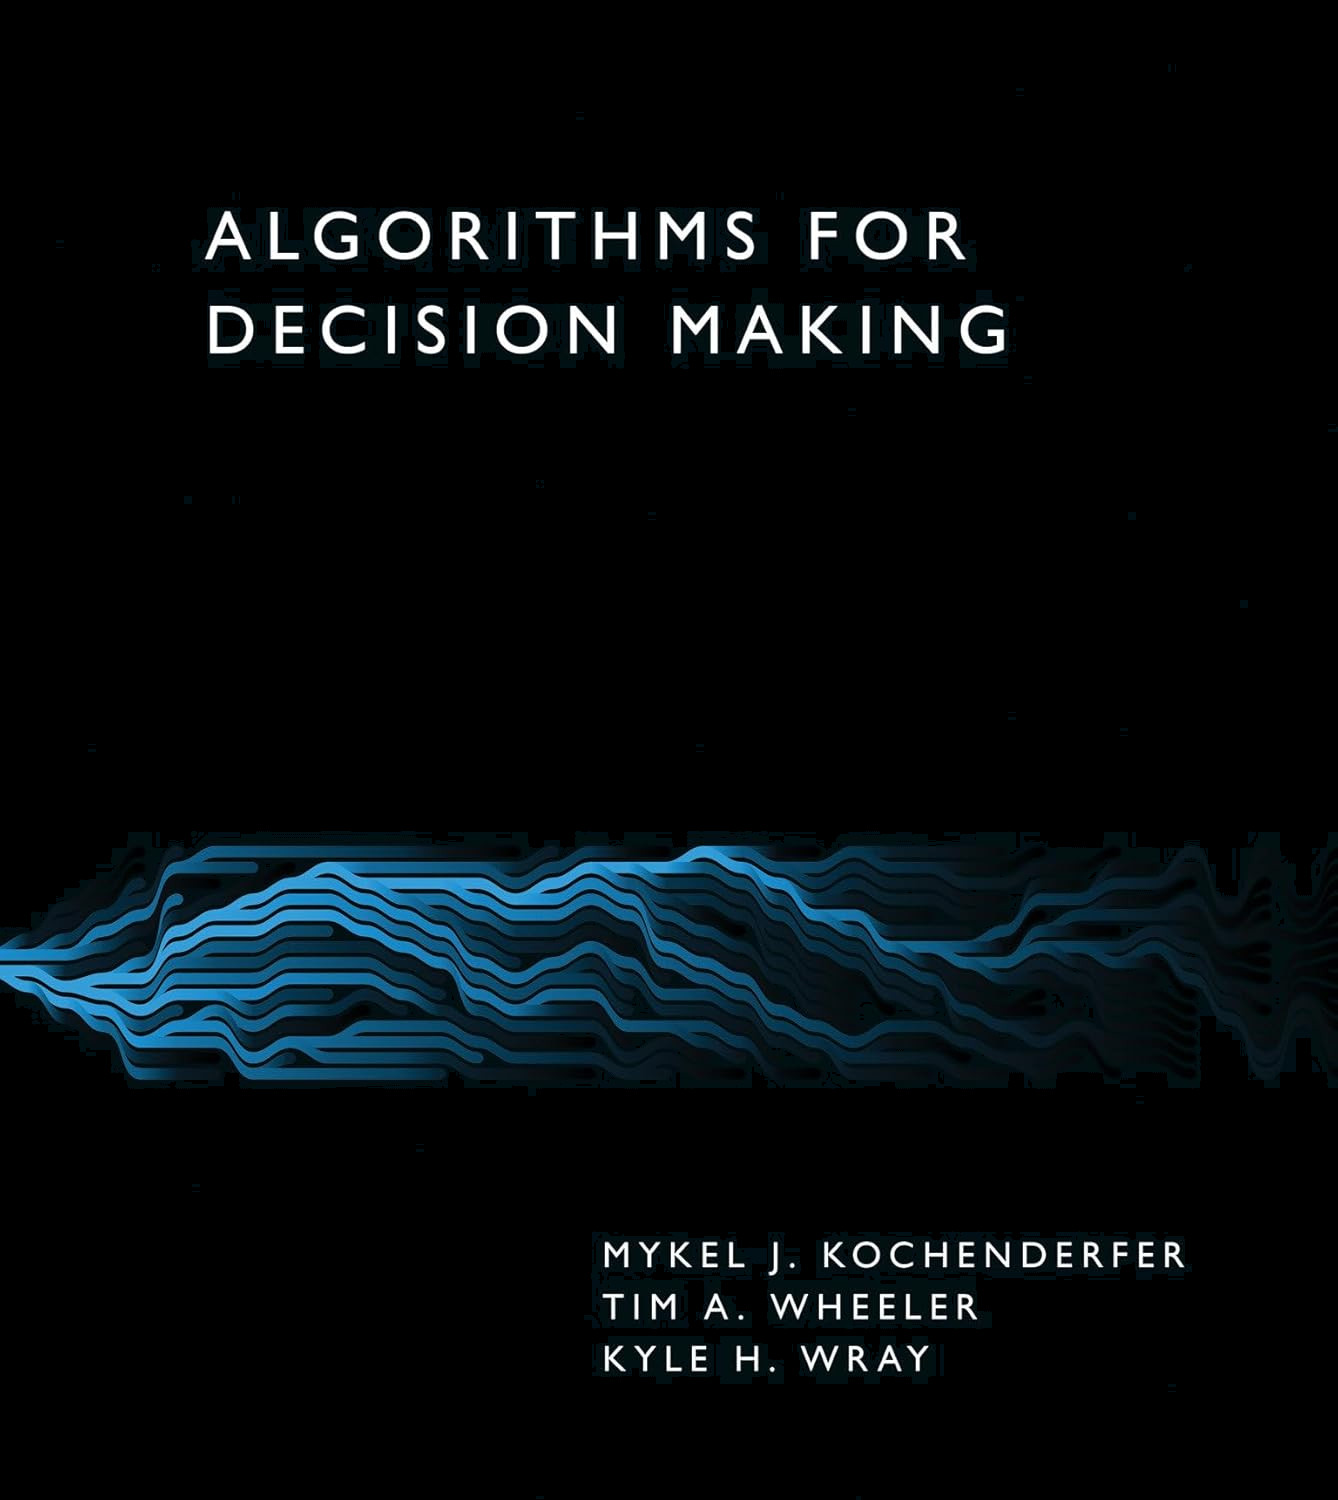
\includegraphics[width=\linewidth]{media/algfordm.png}
        };
    \end{tikzpicture}

    \captionof*{figure}{\shortstack{\footnotesize Algorithms for Decision Making\\\textcolor{gray}{\scriptsize MIT Press, 2022}}}
  \end{column}

  \pause

  \begin{column}{0.30\textwidth}
    \centering
    \begin{tikzpicture}
        \node[draw=white, line width=1pt, inner sep=0pt] {
            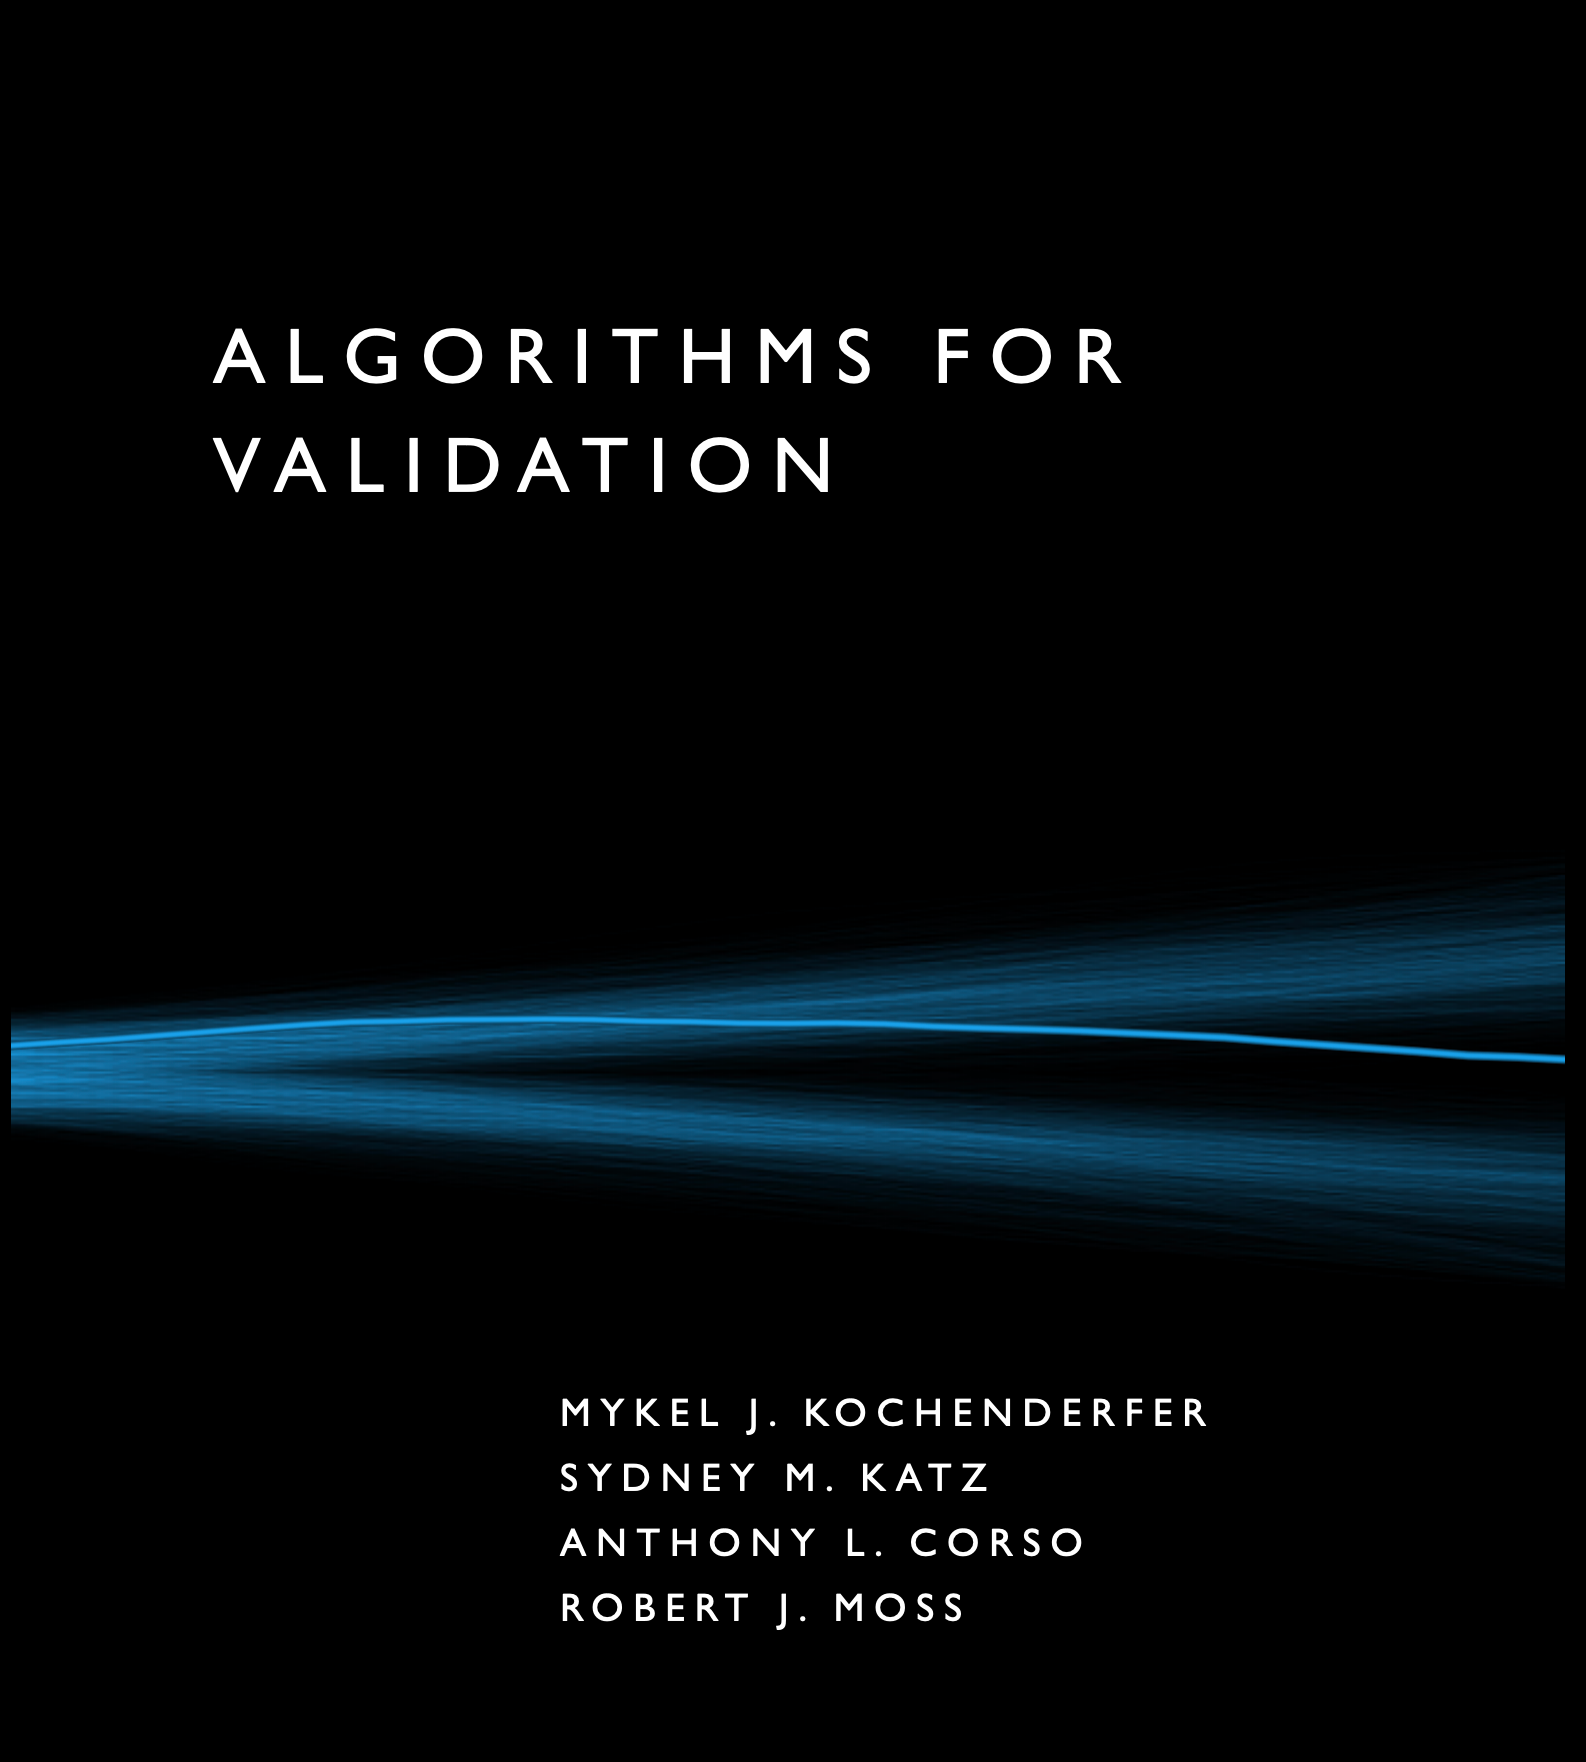
\includegraphics[width=\linewidth]{media/algforval.png}
        };
    \end{tikzpicture}

    \captionof*{figure}{\shortstack{\footnotesize Algorithms for Validation\\\textcolor{gray}{\scriptsize MIT Press, 2025}}}
  \end{column}

\end{columns}

\pause

\small
\centering
All PDFs available for free at \textcolor{repo}{\texttt{https://algorithmsbook.com}}

\end{frame}